
% LaTeX Beamer file automatically generated from DocOnce
% https://github.com/hplgit/doconce

%-------------------- begin beamer-specific preamble ----------------------

\documentclass{beamer}

\usetheme{red_shadow}
\usecolortheme{default}

% turn off the almost invisible, yet disturbing, navigation symbols:
\setbeamertemplate{navigation symbols}{}

% Examples on customization:
%\usecolortheme[named=RawSienna]{structure}
%\usetheme[height=7mm]{Rochester}
%\setbeamerfont{frametitle}{family=\rmfamily,shape=\itshape}
%\setbeamertemplate{items}[ball]
%\setbeamertemplate{blocks}[rounded][shadow=true]
%\useoutertheme{infolines}
%
%\usefonttheme{}
%\useinntertheme{}
%
%\setbeameroption{show notes}
%\setbeameroption{show notes on second screen=right}

% fine for B/W printing:
%\usecolortheme{seahorse}

\usepackage{pgf}
\usepackage{graphicx}
\usepackage{epsfig}
\usepackage{relsize}

\usepackage{fancybox}  % make sure fancybox is loaded before fancyvrb

\usepackage{fancyvrb}
\usepackage{minted} % requires pygments and latex -shell-escape filename
%\usepackage{anslistings}
%\usepackage{listingsutf8}

\usepackage{amsmath,amssymb,bm}
%\usepackage[latin1]{inputenc}
\usepackage[T1]{fontenc}
\usepackage[utf8]{inputenc}
\usepackage{colortbl}
\usepackage[english]{babel}
\usepackage{tikz}
\usepackage{framed}
% Use some nice templates
\beamertemplatetransparentcovereddynamic

% --- begin table of contents based on sections ---
% Delete this, if you do not want the table of contents to pop up at
% the beginning of each section:
% (Only section headings can enter the table of contents in Beamer
% slides generated from DocOnce source, while subsections are used
% for the title in ordinary slides.)
\AtBeginSection[]
{
  \begin{frame}<beamer>[plain]
  \frametitle{}
  %\frametitle{Outline}
  \tableofcontents[currentsection]
  \end{frame}
}
% --- end table of contents based on sections ---

% If you wish to uncover everything in a step-wise fashion, uncomment
% the following command:

%\beamerdefaultoverlayspecification{<+->}

\newcommand{\shortinlinecomment}[3]{\note{\textbf{#1}: #2}}
\newcommand{\longinlinecomment}[3]{\shortinlinecomment{#1}{#2}{#3}}

\definecolor{linkcolor}{rgb}{0,0,0.4}
\hypersetup{
    colorlinks=true,
    linkcolor=linkcolor,
    urlcolor=linkcolor,
    pdfmenubar=true,
    pdftoolbar=true,
    bookmarksdepth=3
    }
\setlength{\parskip}{7pt}  % {1em}

\newenvironment{doconceexercise}{}{}
\newcounter{doconceexercisecounter}
\newenvironment{doconce:movie}{}{}
\newcounter{doconce:movie:counter}

\newcommand{\subex}[1]{\noindent\textbf{#1}}  % for subexercises: a), b), etc

%-------------------- end beamer-specific preamble ----------------------

% Add user's preamble




% insert custom LaTeX commands...

\raggedbottom
\makeindex

%-------------------- end preamble ----------------------

\begin{document}

% matching end for #ifdef PREAMBLE
% #endif

\newcommand{\half}{\frac{1}{2}}
\newcommand{\halfi}{{1/2}}
\newcommand{\tp}{\thinspace .}

\newcommand{\uex}{{u_{\small\mbox{e}}}}
\newcommand{\uexd}[1]{{u_{\small\mbox{e}, #1}}}
\newcommand{\vex}{{v_{\small\mbox{e}}}}
\newcommand{\vexd}[1]{{v_{\small\mbox{e}, #1}}}
\newcommand{\Aex}{{A_{\small\mbox{e}}}}

% Operators
\newcommand{\Ddt}[1]{\frac{D #1}{dt}}
\newcommand{\E}[1]{\hbox{E}\lbrack #1 \rbrack}
\newcommand{\Var}[1]{\hbox{Var}\lbrack #1 \rbrack}
\newcommand{\Std}[1]{\hbox{Std}\lbrack #1 \rbrack}

\newcommand{\xpoint}{\bm{x}}
\newcommand{\normalvec}{\bm{n}}
\newcommand{\Oof}[1]{\mathcal{O}(#1)}

% Boldface vectors/tensors
\newcommand{\x}{\bm{x}}
\newcommand{\X}{\bm{X}}
\renewcommand{\u}{\bm{u}}
\renewcommand{\v}{\bm{v}}
\newcommand{\w}{\bm{w}}
\newcommand{\acc}{\bm{a}}
\newcommand{\rpos}{\bm{r}}
\newcommand{\V}{\bm{V}}
\newcommand{\e}{\bm{e}}
\newcommand{\f}{\bm{f}}
\newcommand{\F}{\bm{F}}
\newcommand{\stress}{\bm{\sigma}}
\newcommand{\strain}{\bm{\varepsilon}}
\newcommand{\stressc}{{\sigma}}
\newcommand{\strainc}{{\varepsilon}}
\newcommand{\I}{\bm{I}}
\newcommand{\T}{\bm{T}}

\newcommand{\dfc}{\alpha}  % diffusion coefficient
% Unit vectors
\newcommand{\ii}{\bm{i}}
\newcommand{\jj}{\bm{j}}
\newcommand{\kk}{\bm{k}}
\newcommand{\ir}{\bm{i}_r}
\newcommand{\ith}{\bm{i}_{\theta}}
\newcommand{\iz}{\bm{i}_z}

% Index sets
\newcommand{\Ix}{\mathcal{I}_x}
\newcommand{\Iy}{\mathcal{I}_y}
\newcommand{\Iz}{\mathcal{I}_z}
\newcommand{\It}{\mathcal{I}_t}
%\newcommand{\Ix}{{I_x}}
%\newcommand{\Iy}{{I_y}}
%\newcommand{\Iz}{{I_z}}
%\newcommand{\It}{{I_t}}
%\newcommand{\If}{\mathcal{I}}     % for FEM
\newcommand{\If}{\mathcal{I}_s}     % for FEM
%\newcommand{\If}{{I}}     % for FEM
%\newcommand{\Ifd}{\mathcal{I}_d}  % for FEM
\newcommand{\Ifd}{{I_d}}  % for FEM
\newcommand{\Ifb}{{I_b}}  % for FEM
\newcommand{\setb}[1]{#1^0}    % set begin
\newcommand{\sete}[1]{#1^{-1}} % set end
%\newcommand{\setl}[1]{#1\setminus\{\set1{#1}\}}
%\newcommand{\setr}[1]{#1\setminus\{\set0{#1}\}}
%\newcommand{\seti}[1]{#1\setminus\{\set0{#1},\set1{#1}\}}
\newcommand{\setl}[1]{#1^-}
\newcommand{\setr}[1]{#1^+}
\newcommand{\seti}[1]{#1^i}
\newcommand{\sequencei}[1]{\left\{ {#1}_i \right\}_{i\in\If}}

% Finite elements
\newcommand{\basphi}{\varphi}
\newcommand{\baspsi}{\psi}
\newcommand{\refphi}{\tilde\basphi}
\newcommand{\psib}{\bm{\psi}}
\newcommand{\sinL}[1]{\sin\left((#1+1)\pi\frac{x}{L}\right)}
\newcommand{\xno}[1]{x_{#1}}
%\newcommand{\xno}[1]{x^{(#1)}}
\newcommand{\Xno}[1]{X_{(#1)}}
\newcommand{\yno}[1]{y_{#1}}
\newcommand{\Yno}[1]{Y_{(#1)}}
\newcommand{\xdno}[1]{\bm{x}_{#1}}

% FEniCS commands
\newcommand{\dX}{\, \mathrm{d}X}
\newcommand{\dx}{\, \mathrm{d}x}
\newcommand{\ds}{\, \mathrm{d}s}
\newcommand{\Real}{\mathbb{R}}
\newcommand{\Integerp}{\mathbb{N}}
\newcommand{\Integer}{\mathbb{Z}}



% ------------------- main content ----------------------



% ----------------- title -------------------------

\title{Study guide: Software engineering with exponential decay models}

% ----------------- author(s) -------------------------

\author{Hans Petter Langtangen\inst{1,2}}
\institute{Center for Biomedical Computing, Simula Research Laboratory\inst{1}
\and
Department of Informatics, University of Oslo\inst{2}}
% ----------------- end author(s) -------------------------

\date{Oct 10, 2015
% <optional titlepage figure>
% <optional copyright>
}

\begin{frame}[plain,fragile]
\titlepage
\end{frame}

\section{From flat program to module with functions}

\begin{frame}[plain,fragile]
\frametitle{Mathematical model problem}

\begin{align*}
u'(t) &= -au(t), \quad t \in (0,T]\\ 
u(0)  &= I
\end{align*}

Solution by $\theta$-scheme:

\begin{equation*}
u^{n+1} = \frac{1 - (1-\theta) a\Delta t}{1 + \theta a\Delta t}u^n
\end{equation*}

$\theta =0$: Forward Euler, $\theta =1$: Backward Euler, $\theta =1/2$: Crank-Nicolson (midpoint method)
\end{frame}

\begin{frame}[plain,fragile]
\frametitle{Many will make a rough, flat program first}

\begin{minted}[fontsize=\fontsize{9pt}{9pt},linenos=false,mathescape,baselinestretch=1.0,fontfamily=tt,xleftmargin=2mm]{python}
from numpy import *
from matplotlib.pyplot import *

A = 1
a = 2
T = 4
dt = 0.2
N = int(round(T/dt))
y = zeros(N+1)
t = linspace(0, T, N+1)
theta = 1
y[0] = A
for n in range(0, N):
    y[n+1] = (1 - (1-theta)*a*dt)/(1 + theta*dt*a)*y[n]

y_e = A*exp(-a*t) - y
error = y_e - y
E = sqrt(dt*sum(error**2))
print 'Norm of the error: %.3E' % E
plot(t, y, 'r--o')
t_e = linspace(0, T, 1001)
y_e = A*exp(-a*t_e)
plot(t_e, y_e, 'b-')
legend(['numerical, theta=%g' % theta, 'exact'])
xlabel('t')
ylabel('y')
show()
\end{minted}
\end{frame}

\begin{frame}[plain,fragile]
\frametitle{There are major issues with this solution}

\begin{enumerate}
\item The notation in the program does not correspond exactly to
   the notation in the mathematical problem: the solution is called
   \texttt{y} and corresponds to $u$ in the mathematical description,
   the variable \texttt{A} corresponds to the mathematical parameter $I$,
   \texttt{N} in the program is called $N_t$ in the mathematics.

\item There are no comments in the program.
\end{enumerate}

\noindent
\end{frame}

\begin{frame}[plain,fragile]
\frametitle{New flat program}

\begin{minted}[fontsize=\fontsize{9pt}{9pt},linenos=false,mathescape,baselinestretch=1.0,fontfamily=tt,xleftmargin=2mm]{python}
from numpy import *
from matplotlib.pyplot import *

I = 1
a = 2
T = 4
dt = 0.2
Nt = int(round(T/dt))     # no of time intervals
u = zeros(Nt+1)           # array of u[n] values
t = linspace(0, T, Nt+1)  # time mesh
theta = 1                 # Backward Euler method

u[0] = I                  # assign initial condition
for n in range(0, Nt):    # n=0,1,...,Nt-1
    u[n+1] = (1 - (1-theta)*a*dt)/(1 + theta*dt*a)*u[n]

# Compute norm of the error
u_e = I*exp(-a*t) - u     # exact u at the mesh points
error = u_e - u
E = sqrt(dt*sum(error**2))
print 'Norm of the error: %.3E' % E

# Compare numerical (u) and exact solution (u_e) in a plot
plot(t, u, 'r--o')
t_e = linspace(0, T, 1001)       # very fine mesh for u_e
u_e = I*exp(-a*t_e)
plot(t_e, u_e, 'b-')
legend(['numerical, theta=%g' % theta, 'exact'])
xlabel('t')
ylabel('u')
show()
\end{minted}
\end{frame}

\begin{frame}[plain,fragile]
\frametitle{Such flat programs are ideal for IPython notebooks!}

% inline figure
\centerline{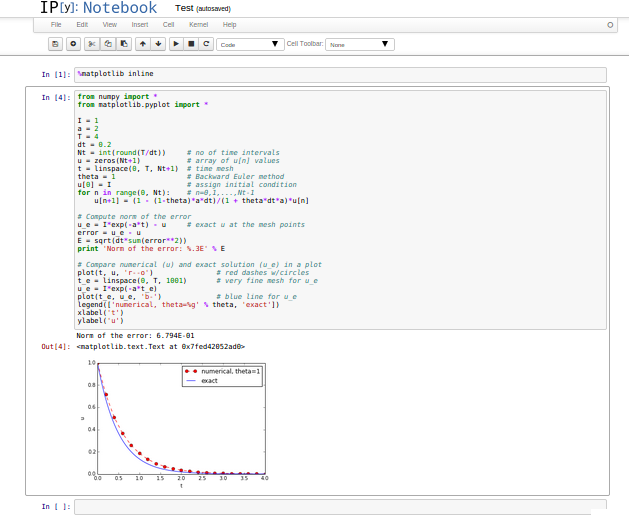
\includegraphics[width=0.9\linewidth]{fig-softeng/ipynb_flat.png}}
\end{frame}

\begin{frame}[plain,fragile]
\frametitle{But: Further development of such flat programs require many scattered edits - easy to make mistakes!}

\begin{center}
\begin{Sbox}
\begin{minipage}{0.85\linewidth}
The solution formula for $u^{n+1}$ is completely general and
should be available as a Python function with all input data as
function arguments and all output data returned to the calling code
\end{minipage}
\end{Sbox}
\fbox{\TheSbox}
\end{center}

\begin{minted}[fontsize=\fontsize{9pt}{9pt},linenos=false,mathescape,baselinestretch=1.0,fontfamily=tt,xleftmargin=2mm]{python}
def solver(I, a, T, dt, theta):
    """Solve u'=-a*u, u(0)=I, for t in (0,T] with steps of dt."""
    dt = float(dt)               # avoid integer division
    Nt = int(round(T/dt))        # no of time intervals
    T = Nt*dt                    # adjust T to fit time step dt
    u = np.zeros(Nt+1)           # array of u[n] values
    t = np.linspace(0, T, Nt+1)  # time mesh

    u[0] = I                  # assign initial condition
    for n in range(0, Nt):    # n=0,1,...,Nt-1
        u[n+1] = (1 - (1-theta)*a*dt)/(1 + theta*dt*a)*u[n]
    return u, t
\end{minted}

Call:

\begin{minted}[fontsize=\fontsize{9pt}{9pt},linenos=false,mathescape,baselinestretch=1.0,fontfamily=tt,xleftmargin=2mm]{python}
u, t = solver(I=1, a=2, T=4, dt=0.2, theta=0.5)
\end{minted}
\end{frame}

\begin{frame}[plain,fragile]
\frametitle{The DRY principle: Don't repeat yourself!}

\begin{block}{DRY: }
When implementing a particular functionality in a computer program, make sure
this functionality and its variations are implemented in just one piece
of code. That is, if you need to revise the implementation, there should be
\emph{one and only one} place to edit. It follows that you should never
duplicate code (don't repeat yourself!), and code snippets that are
similar should be factored into one piece (function) and parameterized (by
function arguments).
\end{block}
\end{frame}

\begin{frame}[plain,fragile]
\frametitle{Make sure any program file is a valid Python module}

\begin{itemize}
 \item Module requires code to be divided into functions :-)

 \item Why module? Other programs can import the functions
\end{itemize}

\noindent
\begin{minted}[fontsize=\fontsize{9pt}{9pt},linenos=false,mathescape,baselinestretch=1.0,fontfamily=tt,xleftmargin=2mm]{python}
from decay import solver
# Solve a decay problem
u, t = solver(I=1, a=2, T=4, dt=0.2, theta=0.5)
\end{minted}
or prefix function names by the module name:

\begin{minted}[fontsize=\fontsize{9pt}{9pt},linenos=false,mathescape,baselinestretch=1.0,fontfamily=tt,xleftmargin=2mm]{python}
import decay
# Solve a decay problem
u, t = decay.solver(I=1, a=2, T=4, dt=0.2, theta=0.5)
\end{minted}
\end{frame}

\begin{frame}[plain,fragile]
\frametitle{The requirements of a module are so simple}

\begin{enumerate}
\item The filename without \texttt{.py} must be a valid Python variable name.

\item The main program must be executed (through statements or
   a function call) in the \emph{test block}.
\end{enumerate}

\noindent
The \emph{test block} is normally placed at the end of a module file:

\begin{minted}[fontsize=\fontsize{9pt}{9pt},linenos=false,mathescape,baselinestretch=1.0,fontfamily=tt,xleftmargin=2mm]{python}
if __name__ == '__main__':
    # Statements
\end{minted}

If the file is imported, the if test fails and no main program is run,
otherwise, the file works as a program
\end{frame}

\begin{frame}[plain,fragile]
\frametitle{The module file \texttt{decay.py} for our example}

\begin{minted}[fontsize=\fontsize{9pt}{9pt},linenos=false,mathescape,baselinestretch=1.0,fontfamily=tt,xleftmargin=2mm]{python}
from numpy import *
from matplotlib.pyplot import *

def solver(I, a, T, dt, theta):
    ...

def u_exact(t, I, a):
    return I*exp(-a*t)

def experiment_compare_numerical_and_exact():
    I = 1;  a = 2;  T = 4;  dt = 0.4;  theta = 1
    u, t = solver(I, a, T, dt, theta)

    t_e = linspace(0, T, 1001)       # very fine mesh for u_e
    u_e = u_exact(t_e, I, a)

    plot(t,   u,   'r--o')           # dashed red line with circles
    plot(t_e, u_e, 'b-')             # blue line for u_e
    legend(['numerical, theta=%g' % theta, 'exact'])
    xlabel('t')
    ylabel('u')
    plotfile = 'tmp'
    savefig(plotfile + '.png');  savefig(plotfile + '.pdf')

    error = u_exact(t, I, a) - u
    E = sqrt(dt*sum(error**2))
    print 'Error norm:', E

if __name__ == '__main__':
    experiment_compare_numerical_and_exact()
\end{minted}

Complete file: \href{{http://tinyurl.com/ofkw6kc/softeng/decay.py}}{\nolinkurl{decay.py}}
\end{frame}

\begin{frame}[plain,fragile]
\frametitle{The module file \texttt{decay.py} for our example w/prefix}

\begin{minted}[fontsize=\fontsize{9pt}{9pt},linenos=false,mathescape,baselinestretch=1.0,fontfamily=tt,xleftmargin=2mm]{python}
import numpy as np
import matplotlib.pyplot as plt

def solver(I, a, T, dt, theta):
    ...

def u_exact(t, I, a):
    return I*np.exp(-a*t)

def experiment_compare_numerical_and_exact():
    I = 1;  a = 2;  T = 4;  dt = 0.4;  theta = 1
    u, t = solver(I, a, T, dt, theta)

    t_e = np.linspace(0, T, 1001)       # very fine mesh for u_e
    u_e = u_exact(t_e, I, a)

    plt.plot(t,   u,   'r--o')       # dashed red line with circles
    plt.plot(t_e, u_e, 'b-')         # blue line for u_e
    plt.legend(['numerical, theta=%g' % theta, 'exact'])
    plt.xlabel('t')
    plt.ylabel('u')
    plotfile = 'tmp'
    plt.savefig(plotfile + '.png');  plt.savefig(plotfile + '.pdf')

    error = u_exact(t, I, a) - u
    E = np.sqrt(dt*np.sum(error**2))
    print 'Error norm:', E

if __name__ == '__main__':
    experiment_compare_numerical_and_exact()
\end{minted}
\end{frame}

\begin{frame}[plain,fragile]
\frametitle{How do we add code for comparing schemes visually?}

% inline figure
\centerline{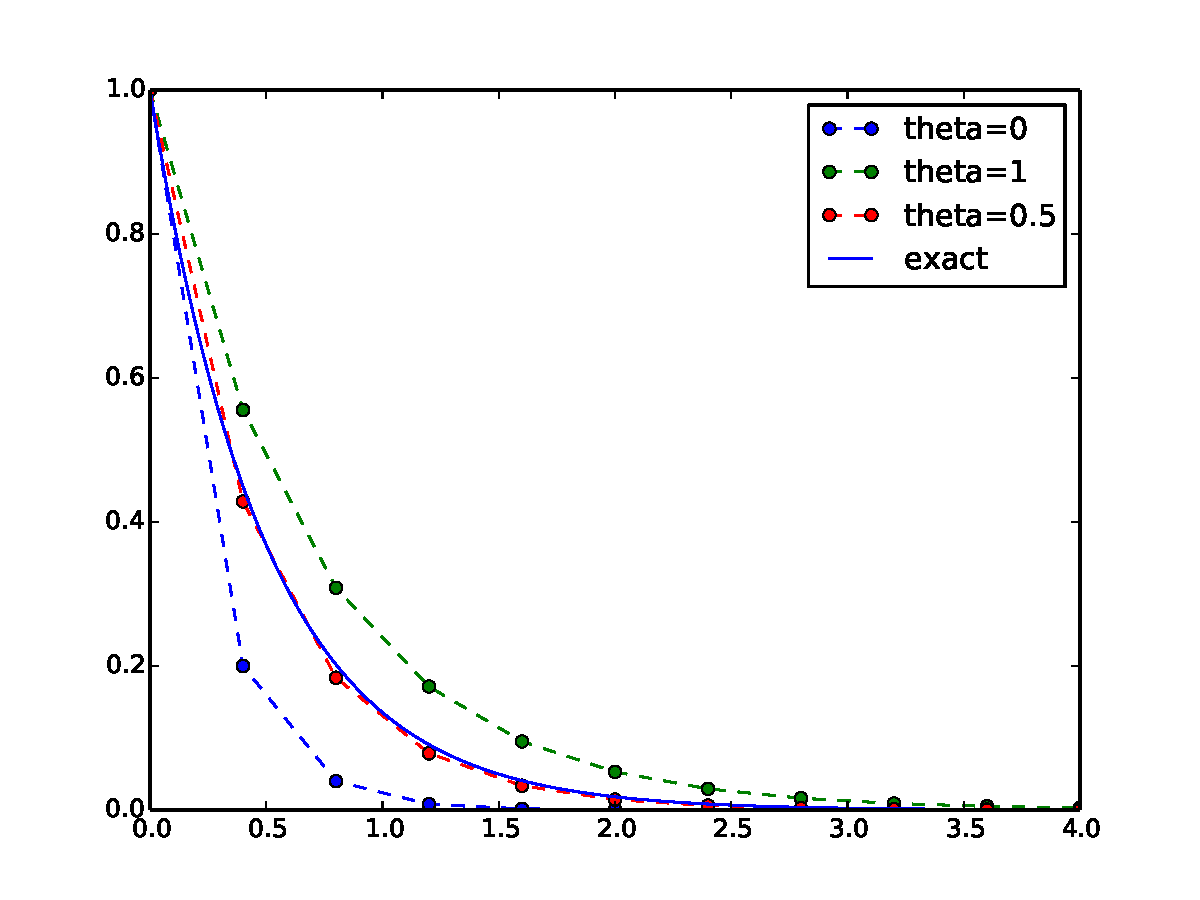
\includegraphics[width=0.9\linewidth]{fig-softeng/compare.pdf}}



Think of edits in the flat program that are required to produce this plot (!)
\end{frame}

\begin{frame}[plain,fragile]
\frametitle{We just add a new function with the tailored plotting}

\begin{minted}[fontsize=\fontsize{9pt}{9pt},linenos=false,mathescape,baselinestretch=1.0,fontfamily=tt,xleftmargin=2mm]{python}
def experiment_compare_schemes():
    """Compare theta=0,1,0.5 in the same plot."""
    I = 1;  a = 2;  T = 4;  dt = 0.4
    legends = []
    for theta in [0, 1, 0.5]:
        u, t = solver(I, a, T, dt, theta)
        plt.plot(t, u, '--o')
        legends.append('theta=%g' % theta)
    t_e = np.linspace(0, T, 1001)        # very fine mesh for u_e
    u_e = u_exact(t_e, I, a)
    plt.plot(t_e, u_e, 'b-')
    legends.append('exact')
    plt.legend(legends, loc='upper right')
    plotfile = 'tmp'
    plt.savefig(plotfile + '.png');  plt.savefig(plotfile + '.pdf')

import logging
logging.basicConfig(
    filename='decay.log', filemode='w', level=logging.DEBUG,
    format='%(asctime)s - %(levelname)s - %(message)s',
    datefmt='%Y.%m.%d %I:%M:%S %p')

def solver_with_logging(I, a, T, dt, theta):
    """Solve u'=-a*u, u(0)=I, for t in (0,T] with steps of dt."""
    dt = float(dt)               # avoid integer division
    Nt = int(round(T/dt))        # no of time intervals
    T = Nt*dt                    # adjust T to fit time step dt
    u = np.zeros(Nt+1)           # array of u[n] values
    t = np.linspace(0, T, Nt+1)  # time mesh
    logging.debug('solver: dt=%g, Nt=%g, T=%g' % (dt, Nt, T))

    u[0] = I                  # assign initial condition
    for n in range(0, Nt):    # n=0,1,...,Nt-1
        u[n+1] = (1 - (1-theta)*a*dt)/(1 + theta*dt*a)*u[n]

        logging.info('u[%d]=%g' % (n, u[n]))
        logging.debug('1 - (1-theta)*a*dt: %g, %s' %
                      (1-(1-theta)*a*dt,
                       str(type(1-(1-theta)*a*dt))[7:-2]))
        logging.debug('1 + theta*dt*a: %g, %s' %
                      (1 + theta*dt*a,
                       str(type(1 + theta*dt*a))[7:-2]))
    return u, t
\end{minted}
\end{frame}

\begin{frame}[plain,fragile]
\frametitle{Prefixing imported functions by the module name}

MATLAB-style names (\texttt{linspace}, \texttt{plot}):

\begin{minted}[fontsize=\fontsize{9pt}{9pt},linenos=false,mathescape,baselinestretch=1.0,fontfamily=tt,xleftmargin=2mm]{python}
from numpy import *
from matplotlib.pyplot import *
\end{minted}

Python community convention is to prefix with module name
(\texttt{np.linspace}, \texttt{plt.plot}):

\begin{minted}[fontsize=\fontsize{9pt}{9pt},linenos=false,mathescape,baselinestretch=1.0,fontfamily=tt,xleftmargin=2mm]{python}
import numpy as np
import matplotlib.pyplot as plt
\end{minted}
\end{frame}

\begin{frame}[plain,fragile]
\frametitle{Documenting functions and modules}

\label{softeng1:basic:docstring}

\begin{itemize}
 \item Use NumPy-style doc strings!

 \item See \href{{https://github.com/numpy/numpy/blob/master/doc/HOWTO_DOCUMENT.rst.txt}}{extensive documentation}

 \item These dominate in the Python scientific computing community

 \item Easy to read with \texttt{pydoc} in the terminal

 \item Can easily autogenerate beautiful online manuals
\end{itemize}

\noindent
\end{frame}

\begin{frame}[plain,fragile]
\frametitle{Example on NumPy-style doc string}

\begin{minted}[fontsize=\fontsize{9pt}{9pt},linenos=false,mathescape,baselinestretch=1.0,fontfamily=tt,xleftmargin=2mm]{python}
def solver(I, a, T, dt, theta):
    """
    Solve :math:`u'=-au` with :math:`u(0)=I` for :math:`t \in (0,T]`
    with steps of `dt` and the method implied by `theta`.

    Parameters
    ----------
    I: float
        Initial condition.
    a: float
        Parameter in the differential equation.
    T: float
        Total simulation time.
    theta: float, int
        Parameter in the numerical scheme. 0 gives
        Forward Euler, 1 Backward Euler, and 0.5
        the centered Crank-Nicolson scheme.

    Returns
    -------
    `u`: array
        Solution array.
    `t`: array
        Array with time points corresponding to `u`.

    Examples
    --------
    Solve :math:`u' = -\\frac{1}{2}u, u(0)=1.5`
    with the Crank-Nicolson method:

    >>> u, t = solver(I=1.5, a=0.5, T=9, theta=0.5)
    >>> import matplotlib.pyplot as plt
    >>> plt.plot(t, u)
    >>> plt.show()
    """
\end{minted}
\end{frame}

\begin{frame}[plain,fragile]
\frametitle{Example on an autogenerated nice HTML manual}

\begin{itemize}
 \item Can use a \href{{http://tinyurl.com/ofkw6kc/softeng/make_sphinx_api.py}}{premade script} to use \href{{http://sphinx-doc.org/}}{Sphinx} to generate an API manual in (e.g.) HTML
\end{itemize}

\noindent
% inline figure
\centerline{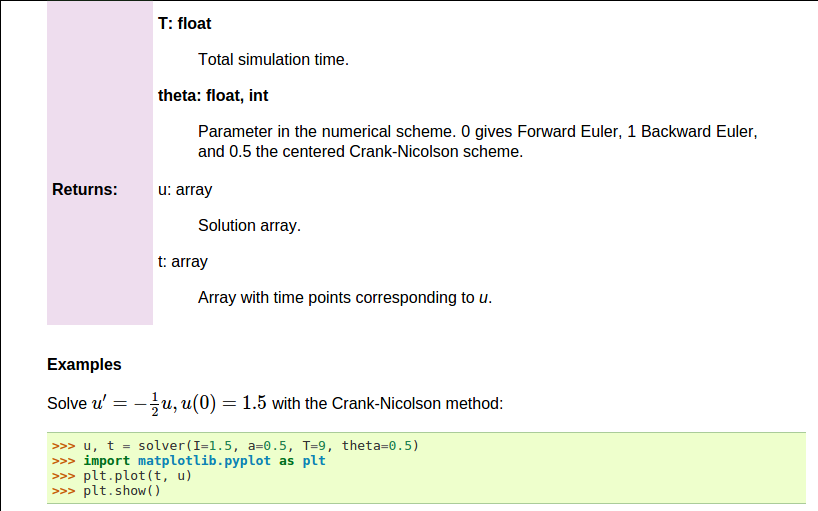
\includegraphics[width=0.8\linewidth]{fig-softeng/selfdoc_numpy.png}}
\end{frame}

\begin{frame}[plain,fragile]
\frametitle{Logging intermediate results}

\label{softeng1:basic:logging}

\begin{itemize}
 \item Simulation programs often have long CPU times

 \item Desire 1: monitor intermediate results/progress

 \item Desire 2: turn on more intermediate results for debugging or troubleshooting
\end{itemize}

\noindent
Most programming languages has a \emph{logging} object for this purpose:

\begin{itemize}
 \item Write messages to a log file

 \item Classify messages as \emph{critical}, \emph{warning}, \emph{info}, or \emph{debug}

 \item Set logging level to one of the four types of messages
\end{itemize}

\noindent
\end{frame}

\begin{frame}[plain,fragile]
\frametitle{Introductory example on using a logger}

\begin{minted}[fontsize=\fontsize{9pt}{9pt},linenos=false,mathescape,baselinestretch=1.0,fontfamily=tt,xleftmargin=2mm]{python}
import logging
import logging
logging.basicConfig(
    filename='myprog.log', filemode='w', level=logging.WARNING,
    format='%(asctime)s - %(levelname)s - %(message)s',
    datefmt='%m/%d/%Y %I:%M:%S %p')
logging.info('Here is some general info.')
logging.warning('Here is a warning.')
logging.debug('Here is some debugging info.')
logging.critical('Dividing by zero!')
logging.error('Encountered an error.')
\end{minted}

Output in \texttt{myprog.log}:

\begin{minted}[fontsize=\fontsize{9pt}{9pt},linenos=false,mathescape,baselinestretch=1.0,fontfamily=tt,xleftmargin=2mm]{text}
09/26/2015 09:25:10 AM - INFO - Here is some general info.
09/26/2015 09:25:10 AM - WARNING - Here is a warning.
09/26/2015 09:25:10 AM - CRITICAL - Dividing by zero!
09/26/2015 09:25:10 AM - ERROR - Encountered an error.
\end{minted}
\end{frame}

\begin{frame}[plain,fragile]
\frametitle{A message is tied to a level, and one can specify one many levels that get printed}

Levels: critical, error, warning, info, debug

\begin{enumerate}
\item \texttt{level=logging.CRITICAL}: print critical messages

\item \texttt{level=logging.ERROR}: print critical and error messages

\item \texttt{level=logging.WARNING}: print critical, error, and warning messages

\item \texttt{level=logging.INFO}: print critical, error, warning, and info messages

\item \texttt{level=logging.DEBUG}: print critical, error, warning, info, and debug messages
\end{enumerate}

\noindent
\end{frame}

\begin{frame}[plain,fragile]
\frametitle{Using a logger in our solver function}

\begin{minted}[fontsize=\fontsize{9pt}{9pt},linenos=false,mathescape,baselinestretch=1.0,fontfamily=tt,xleftmargin=2mm]{python}
import logging
logging.basicConfig(
    filename='decay.log', filemode='w', level=logging.DEBUG,
    format='%(asctime)s - %(levelname)s - %(message)s',
    datefmt='%Y.%m.%d %I:%M:%S %p')

def solver_with_logging(I, a, T, dt, theta):
    """Solve u'=-a*u, u(0)=I, for t in (0,T] with steps of dt."""
    dt = float(dt)               # avoid integer division
    Nt = int(round(T/dt))        # no of time intervals
    T = Nt*dt                    # adjust T to fit time step dt
    u = np.zeros(Nt+1)           # array of u[n] values
    t = np.linspace(0, T, Nt+1)  # time mesh
    logging.debug('solver: dt=%g, Nt=%g, T=%g' % (dt, Nt, T))

    u[0] = I                  # assign initial condition
    for n in range(0, Nt):    # n=0,1,...,Nt-1
        u[n+1] = (1 - (1-theta)*a*dt)/(1 + theta*dt*a)*u[n]

        logging.info('u[%d]=%g' % (n, u[n]))
        logging.debug('1 - (1-theta)*a*dt: %g, %s' %
                      (1-(1-theta)*a*dt,
                       str(type(1-(1-theta)*a*dt))[7:-2]))
        logging.debug('1 + theta*dt*a: %g, %s' %
                      (1 + theta*dt*a,
                       str(type(1 + theta*dt*a))[7:-2]))
    return u, t
\end{minted}
\end{frame}

\begin{frame}[plain,fragile]
\frametitle{Monitoring messages}

One terminal window (1M steps!):

\begin{minted}[fontsize=\fontsize{9pt}{9pt},linenos=false,mathescape,baselinestretch=1.0,fontfamily=tt,xleftmargin=2mm]{python}
>>> import decay
>>> u, t = decay.solver_with_logging(I=1, a=0.5, T=10, \ 
           dt=0.5, theta=0.5)
\end{minted}

Another terminal window:

\begin{minted}[fontsize=\fontsize{9pt}{9pt},linenos=false,mathescape,baselinestretch=1.0,fontfamily=tt,xleftmargin=2mm]{console}
Terminal> tail -f decay.log
2015.09.26 05:37:41 AM - INFO - u[0]=1
2015.09.26 05:37:41 AM - INFO - u[1]=0.777778
2015.09.26 05:37:41 AM - INFO - u[2]=0.604938
2015.09.26 05:37:41 AM - INFO - u[3]=0.470508
2015.09.26 05:37:41 AM - INFO - u[4]=0.36595
2015.09.26 05:37:41 AM - INFO - u[5]=0.284628
\end{minted}

Or if \texttt{level=logging.DEBUG}:

\begin{minted}[fontsize=\fontsize{9pt}{9pt},linenos=false,mathescape,baselinestretch=1.0,fontfamily=tt,xleftmargin=2mm]{console}
Terminal> tail -f decay.log
2015.09.26 05:40:01 AM - DEBUG - solver: dt=0.5, Nt=20, T=10
2015.09.26 05:40:01 AM - INFO - u[0]=1
2015.09.26 05:40:01 AM - DEBUG - 1 - (1-theta)*a*dt: 0.875, float
2015.09.26 05:40:01 AM - DEBUG - 1 + theta*dt*a: 1.125, float
2015.09.26 05:40:01 AM - INFO - u[1]=0.777778
2015.09.26 05:40:01 AM - DEBUG - 1 - (1-theta)*a*dt: 0.875, float
2015.09.26 05:40:01 AM - DEBUG - 1 + theta*dt*a: 1.125, float
\end{minted}
\end{frame}

\section{User interfaces}

\begin{frame}[plain,fragile]
\frametitle{User interfaces}

\label{decay:GUI}

\begin{itemize}
 \item Never edit the program to change input!

 \item Set input data on the command line or in a graphical user interface

 \item How is explained next
\end{itemize}

\noindent

\end{frame}

\begin{frame}[plain,fragile]
\frametitle{Accessing command-line arguments}

\begin{itemize}
 \item All command-line arguments are available in \texttt{sys.argv}

 \item \texttt{sys.argv[0]} is the program

 \item \texttt{sys.argv[1:]} holds the command-line arguments

 \item Method 1: fixed sequence of parameters on the command line

 \item Method 2: \texttt{--option value} pairs on the command line (with default values)
\end{itemize}

\noindent
\begin{minted}[fontsize=\fontsize{9pt}{9pt},linenos=false,mathescape,baselinestretch=1.0,fontfamily=tt,xleftmargin=2mm]{console}
Terminal> python myprog.py 1.5 2 0.5 0.8 0.4
Terminal> python myprog.py --I 1.5 --a 2 --dt 0.8 0.4
\end{minted}
\end{frame}

\begin{frame}[plain,fragile]
\frametitle{Reading a sequence of command-line arguments}

Required input:

\begin{itemize}
 \item $I$

 \item $a$

 \item $T$

 \item name of scheme (FE, BE, CN)

 \item a list of $\Delta t$ values
\end{itemize}

\noindent
Give these on the command line in correct sequence

\begin{minted}[fontsize=\fontsize{9pt}{9pt},linenos=false,mathescape,baselinestretch=1.0,fontfamily=tt,xleftmargin=2mm]{console}
Terminal> python decay_cml.py 1.5 0.5 4 CN 0.1 0.2 0.05
\end{minted}
\end{frame}

\begin{frame}[plain,fragile]
\frametitle{Implementation}

\begin{minted}[fontsize=\fontsize{9pt}{9pt},linenos=false,mathescape,baselinestretch=1.0,fontfamily=tt,xleftmargin=2mm]{python}
def define_command_line_options():
    import argparse
    parser = argparse.ArgumentParser()
    parser.add_argument(
        '--I', '--initial_condition', type=float,
        default=1.0, help='initial condition, u(0)',
        metavar='I')
    parser.add_argument(
        '--a', type=float, default=1.0,
        help='coefficient in ODE', metavar='a')
    parser.add_argument(
        '--T', '--stop_time', type=float,
        default=1.0, help='end time of simulation',
        metavar='T')
    parser.add_argument(
        '--scheme', type=str, default='CN',
        help='FE, BE, or CN')
    parser.add_argument(
        '--dt', '--time_step_values', type=float,
        default=[1.0], help='time step values',
        metavar='dt', nargs='+', dest='dt_values')
    return parser
\end{minted}

Note:

\begin{itemize}
  \item \texttt{sys.argv[i]} is \emph{always a string}

  \item Must explicitly convert to (e.g.) \texttt{float} for computations

  \item List comprehensions make lists: \texttt{[expression for e in somelist]}
\end{itemize}

\noindent
\end{frame}

\begin{frame}[plain,fragile]
\frametitle{Working with an argument parser}

Set option-value pairs on the command line if the default value is not
suitable:

\begin{minted}[fontsize=\fontsize{9pt}{9pt},linenos=false,mathescape,baselinestretch=1.0,fontfamily=tt,xleftmargin=2mm]{console}
Terminal> python decay_argparse.py --I 1.5 --a 2 --dt 0.8 0.4
\end{minted}

Code:

\begin{minted}[fontsize=\fontsize{9pt}{9pt},linenos=false,mathescape,baselinestretch=1.0,fontfamily=tt,xleftmargin=2mm]{python}
def read_command_line_argparse():
    parser = define_command_line_options()
    args = parser.parse_args()
    scheme2theta = {'BE': 1, 'CN': 0.5, 'FE': 0}
    data = (args.I, args.a, args.T, scheme2theta[args.scheme],
            args.dt_values)
    return data
\end{minted}

(\texttt{metavar} is the symbol used in help output)
\end{frame}

\begin{frame}[plain,fragile]
\frametitle{A graphical user interface}

% inline figure
\centerline{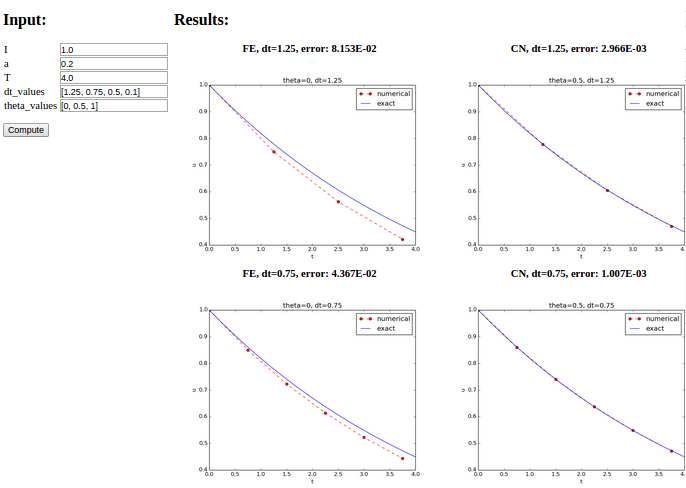
\includegraphics[width=1.0\linewidth]{fig-softeng/web_GUI.png}}



Normally very much programming required - and much competence on
graphical user interfaces.

Here: use a tool to automatically create it in a few minutes (!)
\end{frame}

\begin{frame}[plain,fragile]
\frametitle{The Parampool package}

\begin{itemize}
 \item \href{{https://github.com/hplgit/parampool}}{Parampool} is a package
   for handling a large pool of input parameters in simulation programs

 \item Parampool can automatically create a sophisticated web-based
   graphical user interface (GUI) to set parameters and view solutions
\end{itemize}

\noindent
\begin{block}{Remark }
The forthcoming material aims at those with particular interest in
equipping their programs with a GUI - others can safely skip it.
\end{block}
\end{frame}

\begin{frame}[plain,fragile]
\frametitle{Making a compute function}

\begin{itemize}
 \item Key concept: a \emph{compute function} that takes all input data as arguments
   and returning HTML code for viewing the results (e.g., plots and numbers)

 \item What we have: \href{{http://tinyurl.com/ofkw6kc/softeng/decay_plot.py}}{\nolinkurl{decay_plot.py}}

 \item \texttt{main} function carries out simulations and plotting for a
   series of $\Delta t$ values

 \item Goal: steer and view these experiments from a web GUI

 \item What to do:
\begin{itemize}

   \item create a compute function

   \item call \texttt{parampool} functionality
\end{itemize}

\noindent
\end{itemize}

\noindent
\end{frame}

\begin{frame}[plain,fragile]
\frametitle{The compute function must return HTML code}

\begin{minted}[fontsize=\fontsize{9pt}{9pt},linenos=false,mathescape,baselinestretch=1.0,fontfamily=tt,xleftmargin=2mm]{python}
def main_GUI(I=1.0, a=.2, T=4.0,
             dt_values=[1.25, 0.75, 0.5, 0.1],
             theta_values=[0, 0.5, 1]):
    # Build HTML code for web page. Arrange plots in columns
    # corresponding to the theta values, with dt down the rows
    theta2name = {0: 'FE', 1: 'BE', 0.5: 'CN'}
    html_text = '<table>\n'
    for dt in dt_values:
        html_text += '<tr>\n'
        for theta in theta_values:
            E, html = compute4web(I, a, T, dt, theta)
            html_text += """
<td>
<center><b>%s, dt=%g, error: %.3E</b></center><br>
%s
</td>
""" % (theta2name[theta], dt, E, html)
        html_text += '</tr>\n'
    html_text += '</table>\n'
    return html_text
\end{minted}
\end{frame}

\begin{frame}[plain,fragile]
\frametitle{Generating the user interface}

Make a file \Verb!decay_GUI_generate.py!:

\begin{minted}[fontsize=\fontsize{9pt}{9pt},linenos=false,mathescape,baselinestretch=1.0,fontfamily=tt,xleftmargin=2mm]{python}
from parampool.generator.flask import generate
from decay import main_GUI
generate(main_GUI,
         filename_controller='decay_GUI_controller.py',
         filename_template='decay_GUI_view.py',
         filename_model='decay_GUI_model.py')
\end{minted}

Running \Verb!decay_GUI_generate.py! results in

\begin{enumerate}
 \item \Verb!decay_GUI_model.py! defines HTML widgets to be used to set
    input data in the web interface,

 \item \Verb!templates/decay_GUI_views.py! defines the layout of the web page,

 \item \Verb!decay_GUI_controller.py! runs the web application.
\end{enumerate}

\noindent
Good news: we only need to run \Verb!decay_GUI_controller.py!
and there is no need to look into any of these files!
\end{frame}

\begin{frame}[plain,fragile]
\frametitle{Running the web application}

Start the GUI

\begin{minted}[fontsize=\fontsize{9pt}{9pt},linenos=false,mathescape,baselinestretch=1.0,fontfamily=tt,xleftmargin=2mm]{console}
Terminal> python decay_GUI_controller.py
\end{minted}
Open a web browser at \texttt{127.0.0.1:5000}



% inline figure
\centerline{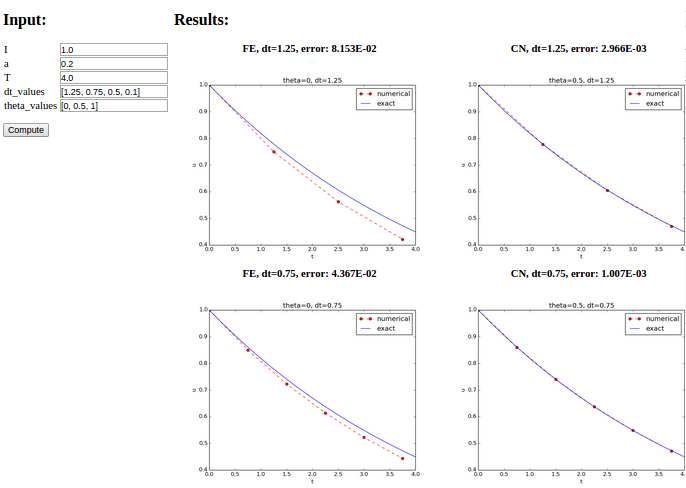
\includegraphics[width=1.0\linewidth]{fig-softeng/web_GUI.png}}
\end{frame}

\begin{frame}[plain,fragile]
\frametitle{More advanced use}

\begin{itemize}
 \item The compute function can have arguments of type float, int, string,
   list, dict, numpy array, filename (file upload)

 \item Alternative: specify a hierarchy of input parameters with name,
   default value, data type, widget type, unit (m, kg, s), validity check

 \item The generated web GUI can have user accounts with login and storage
   of results in a database
\end{itemize}

\noindent
\end{frame}

\section{Tests for verifying implementations}

\begin{frame}[plain,fragile]
\frametitle{Doctests}

\index{doctests}
\index{software testing!doctests}

Doc strings can be equipped with interactive Python sessions for
demonstrating usage and \emph{automatic testing} of functions.

\begin{minted}[fontsize=\fontsize{9pt}{9pt},linenos=false,mathescape,baselinestretch=1.0,fontfamily=tt,xleftmargin=2mm]{python}
def solver(I, a, T, dt, theta):
    """
    Solve u'=-a*u, u(0)=I, for t in (0,T] with steps of dt.


    >>> u, t = solver(I=0.8, a=1.2, T=2, dt=0.5, theta=0.5)
    >>> for t_n, u_n in zip(t, u):
    ...     print 't=%.1f, u=%.14f' % (t_n, u_n)
    t=0.0, u=0.80000000000000
    t=0.5, u=0.43076923076923
    t=1.0, u=0.23195266272189
    t=1.5, u=0.12489758761948
    t=2.0, u=0.06725254717972
    """
    ...
\end{minted}
\end{frame}

\begin{frame}[plain,fragile]
\frametitle{Running doctests}

Automatic check that the code reproduces the doctest output:

\begin{minted}[fontsize=\fontsize{9pt}{9pt},linenos=false,mathescape,baselinestretch=1.0,fontfamily=tt,xleftmargin=2mm]{python}
Terminal> python -m doctest decay.py
\end{minted}

\begin{block}{Floats are difficult to compare }
Limit the number of digits in the output in doctests! Otherwise,
round-off errors on a different machine may ruin the test.
\end{block}
\end{frame}

\begin{frame}[plain,fragile]
\frametitle{Unit testing with nose}

\index{nose@{\rm\texttt{nose}} testing}
\index{unit testing}
\index{software testing!nose}

\begin{itemize}
 \item Nose and pytest are a very user-friendly testing frameworks

 \item Based on \emph{unit testing}

 \item Identify (small) units of code and test each unit

 \item Nose automates running all tests

 \item Good habit: run all tests after (small) edits of a code

 \item Even better habit: write tests \emph{before} the code (!)

 \item Remark: unit testing in scientific computing is not yet well established
\end{itemize}

\noindent
\end{frame}

\begin{frame}[plain,fragile]
\frametitle{Basic use of nose and pytest}

\begin{enumerate}
 \item Implement tests in \emph{test functions} with names starting with \Verb!test_!.

 \item Test functions cannot have arguments.

 \item Test functions perform assertions on computed results
    using \texttt{assert} functions from the \texttt{nose.tools} module.

 \item Test functions can be in the source code files or be
    collected in separate files \texttt{test*.py}.
\end{enumerate}

\noindent
\end{frame}

\begin{frame}[plain,fragile]
\frametitle{Example on a test function in the source code}

Very simple module \texttt{mymod} (in file \texttt{mymod.py}):

\begin{minted}[fontsize=\fontsize{9pt}{9pt},linenos=false,mathescape,baselinestretch=1.0,fontfamily=tt,xleftmargin=2mm]{python}
def double(n):
    return 2*n
\end{minted}

Write test function in \texttt{mymod.py}:

\begin{minted}[fontsize=\fontsize{9pt}{9pt},linenos=false,mathescape,baselinestretch=1.0,fontfamily=tt,xleftmargin=2mm]{python}
def double(n):
    return 2*n

def test_double():
    n = 4
    expected = 2*4
    computed = double(n)
    assert expected == computed
\end{minted}

Running one of

\begin{minted}[fontsize=\fontsize{9pt}{9pt},linenos=false,mathescape,baselinestretch=1.0,fontfamily=tt,xleftmargin=2mm]{console}
Terminal> nosetests -s -v mymod
Terminal> py.test   -s -v mymod
\end{minted}
makes the framework run all \Verb!test_*()! functions in \texttt{mymod.py}.
\end{frame}

\begin{frame}[plain,fragile]
\frametitle{Example on test functions in a separate file}

Write the test in a separate file, say \Verb!test_mymod.py!:

\begin{minted}[fontsize=\fontsize{9pt}{9pt},linenos=false,mathescape,baselinestretch=1.0,fontfamily=tt,xleftmargin=2mm]{python}
import mymod

def test_double():
    n = 4
    expected = 2*4
    computed = double(n)
    assert expected == computed
\end{minted}

Running one of

\begin{minted}[fontsize=\fontsize{9pt}{9pt},linenos=false,mathescape,baselinestretch=1.0,fontfamily=tt,xleftmargin=2mm]{console}
Terminal> nosetests -s -v
Terminal> py.test   -s -v
\end{minted}
makes the frameworks run all \Verb!test_*()! functions in all files
\texttt{test*.py} in the current directory and in all subdirectories (pytest)
or just those with names \texttt{tests} or \Verb!*_tests! (nose)

\begin{block}{Tip }
Start with test functions in the source code file. When the file
contains many tests, or when you have many source code files,
move tests to separate files.
\end{block}
\end{frame}

\begin{frame}[plain,fragile]
\frametitle{Test function for solver}

Use exact discrete solution of the $\theta$ scheme as test:

\[ u^n = I\left(
\frac{1 - (1-\theta) a\Delta t}{1 + \theta a \Delta t}
\right)^n\]

\begin{minted}[fontsize=\fontsize{9pt}{9pt},linenos=false,mathescape,baselinestretch=1.0,fontfamily=tt,xleftmargin=2mm]{python}
def u_discrete_exact(n, I, a, theta, dt):
    """Return exact discrete solution of the numerical schemes."""
    dt = float(dt)  # avoid integer division
    A = (1 - (1-theta)*a*dt)/(1 + theta*dt*a)
    return I*A**n
\end{minted}

\begin{minted}[fontsize=\fontsize{9pt}{9pt},linenos=false,mathescape,baselinestretch=1.0,fontfamily=tt,xleftmargin=2mm]{python}
def test_u_discrete_exact():
    """Check that solver reproduces the exact discr. sol."""
    theta = 0.8; a = 2; I = 0.1; dt = 0.8
    Nt = int(8/dt)  # no of steps
    u, t = solver(I=I, a=a, T=Nt*dt, dt=dt, theta=theta)

    # Evaluate exact discrete solution on the mesh
    u_de = np.array([u_discrete_exact(n, I, a, theta, dt)
                     for n in range(Nt+1)])

    # Find largest deviation
    diff = np.abs(u_de - u).max()
    tol = 1E-14
    success = diff < tol
    assert success
\end{minted}
\end{frame}

\begin{frame}[plain,fragile]
\frametitle{Can test that potential integer division is avoided too}

\begin{block}{Warning}
If $a$, $\Delta t$, and
$\theta$ are integers, the formula for $u^{n+1}$ in the solver
function may lead to 0 because of unintended integer division.
\end{block}

\begin{minted}[fontsize=\fontsize{9pt}{9pt},linenos=false,mathescape,baselinestretch=1.0,fontfamily=tt,xleftmargin=2mm]{python}
def test_potential_integer_division():
    """Choose variables that can trigger integer division."""
    theta = 1; a = 1; I = 1; dt = 2
    Nt = 4
    u, t = solver(I=I, a=a, T=Nt*dt, dt=dt, theta=theta)
    u_de = np.array([u_discrete_exact(n, I, a, theta, dt)
                     for n in range(Nt+1)])
    diff = np.abs(u_de - u).max()
    assert diff < 1E-14
\end{minted}
\end{frame}

\section{Packaging the software for other users}

\begin{frame}[plain,fragile]
\frametitle{Packaging the software for other users}




Installation of a single module file \texttt{decay.py}:

\begin{minted}[fontsize=\fontsize{9pt}{9pt},linenos=false,mathescape,baselinestretch=1.0,fontfamily=tt,xleftmargin=2mm]{python}
from distutils.core import setup
setup(name='decay',
      version='0.1',
      py_modules=['decay'],
      scripts=['decay.py'],
      )
\end{minted}

Installation:

\begin{minted}[fontsize=\fontsize{9pt}{9pt},linenos=false,mathescape,baselinestretch=1.0,fontfamily=tt,xleftmargin=2mm]{console}
Terminal> sudo python setup.py install
\end{minted}

(Many variants!)


\end{frame}

\begin{frame}[plain,fragile]
\frametitle{split.py for several modules in a package}

\begin{itemize}
 \item Python package = several modules

 \item Modules be in a directory with a \Verb!__init__.py! file

 \item Name of package = name of directory
\end{itemize}

\noindent
\texttt{setup.py}:

\begin{minted}[fontsize=\fontsize{9pt}{9pt},linenos=false,mathescape,baselinestretch=1.0,fontfamily=tt,xleftmargin=2mm]{python}
from distutils.core import setup
import os

setup(name='decay',
      version='0.1',
      author='Hans Petter Langtangen',
      author_email='hpl@simula.no',
      url='https://github.com/hplgit/decay-package/',
      packages=['decay'],
      scripts=[os.path.join('decay', 'decay.py')]
     )
\end{minted}
\end{frame}

\begin{frame}[plain,fragile]
\frametitle{The \protect\Verb!\_\_init\_\_.py! file can be empty}

Empty \Verb!__init__.py!:

\begin{minted}[fontsize=\fontsize{9pt}{9pt},linenos=false,mathescape,baselinestretch=1.0,fontfamily=tt,xleftmargin=2mm]{text}
import decay
u, t = decay.decay.solver(...)
\end{minted}

Do this in \Verb!__init__.py! to avoid \texttt{decay.decay.solver}:

\begin{minted}[fontsize=\fontsize{9pt}{9pt},linenos=false,mathescape,baselinestretch=1.0,fontfamily=tt,xleftmargin=2mm]{python}
from decay import *
\end{minted}

Can now write

\begin{minted}[fontsize=\fontsize{9pt}{9pt},linenos=false,mathescape,baselinestretch=1.0,fontfamily=tt,xleftmargin=2mm]{text}
import decay
u, t = decay.solver(...)

# or
from decay import solver
u, t = solver(...)
\end{minted}
\end{frame}

\begin{frame}[plain,fragile]
\frametitle{Always develop software and write reports with Git}

\begin{itemize}
 \item Git keeps track of different versions of files

 \item Can roll back to previous versions

 \item Can see who did what when

 \item Can merge simultaneous edits by different users

 \item Professionals rely on Git!
\end{itemize}

\noindent
The Git work cycle:

\begin{minted}[fontsize=\fontsize{9pt}{9pt},linenos=false,mathescape,baselinestretch=1.0,fontfamily=tt,xleftmargin=2mm]{text}
git pull                # before starting a new session
# edit files
git add mynewfile       # remember to add new files!
git commit -am 'Short description of what I did'
git push origin master  # before end of day or a break
\end{minted}
\end{frame}

\begin{frame}[plain,fragile]
\frametitle{More pro use with Git}

See what others have done in the project:

\begin{minted}[fontsize=\fontsize{9pt}{9pt},linenos=false,mathescape,baselinestretch=1.0,fontfamily=tt,xleftmargin=2mm]{text}
git fetch origin         # instead of git pull
git diff origin/master   # what are the changes?
git merge origin/master  # update my files
\end{minted}

Develop new features in a separate branch:

\begin{minted}[fontsize=\fontsize{9pt}{9pt},linenos=false,mathescape,baselinestretch=1.0,fontfamily=tt,xleftmargin=2mm]{text}
git branch newstuff
git checkout newstuff
# edit files
git commit -am 'Changed ...'
git push origin newstuff
\end{minted}
When \texttt{newstuff} is tested and matured, merge back in master:

\begin{minted}[fontsize=\fontsize{9pt}{9pt},linenos=false,mathescape,baselinestretch=1.0,fontfamily=tt,xleftmargin=2mm]{text}
git checkout master
git merge newstuff
\end{minted}
\end{frame}

\section{Classes for problem and solution method}
\label{softeng1:prog:se:class}

\begin{frame}[plain,fragile]
\frametitle{Collect physical problem and parameters in class Problem}

\begin{minted}[fontsize=\fontsize{9pt}{9pt},linenos=false,mathescape,baselinestretch=1.0,fontfamily=tt,xleftmargin=2mm]{python}
from numpy import exp

class Problem(object):
    def __init__(self, I=1, a=1, T=10):
        self.T, self.I, self.a = I, float(a), T

    def u_exact(self, t):
        I, a = self.I, self.a
        return I*exp(-a*t)
\end{minted}
\end{frame}

\begin{frame}[plain,fragile]
\frametitle{Collect numerical parameters and methods in class Solver}

\begin{minted}[fontsize=\fontsize{9pt}{9pt},linenos=false,mathescape,baselinestretch=1.0,fontfamily=tt,xleftmargin=2mm]{python}
class Solver(object):
    def __init__(self, problem, dt=0.1, theta=0.5):
        self.problem = problem
        self.dt, self.theta = float(dt), theta

    def solve(self):
        self.u, self.t = solver(
            self.problem.I, self.problem.a, self.problem.T,
            self.dt, self.theta)

    def error(self):
        """Return norm of error at the mesh points."""
        u_e = self.problem.u_exact(self.t)
        e = u_e - self.u
        E = np.sqrt(self.dt*np.sum(e**2))
        return E
\end{minted}
\end{frame}

\begin{frame}[plain,fragile]
\frametitle{Get input from the command line; class Problem}

\begin{minted}[fontsize=\fontsize{9pt}{9pt},linenos=false,mathescape,baselinestretch=1.0,fontfamily=tt,xleftmargin=2mm]{python}
class Problem(object):
    def __init__(self, I=1, a=1, T=10):
        self.T, self.I, self.a = I, float(a), T

    def define_command_line_options(self, parser=None):
        """Return updated (parser) or new ArgumentParser object."""
        if parser is None:
            import argparse
            parser = argparse.ArgumentParser()

        parser.add_argument(
            '--I', '--initial_condition', type=float,
            default=1.0, help='initial condition, u(0)',
            metavar='I')
        parser.add_argument(
            '--a', type=float, default=1.0,
            help='coefficient in ODE', metavar='a')
        parser.add_argument(
            '--T', '--stop_time', type=float,
            default=1.0, help='end time of simulation',
            metavar='T')
        return parser

    def init_from_command_line(self, args):
        """Load attributes from ArgumentParser into instance."""
        self.I, self.a, self.T = args.I, args.a, args.T
\end{minted}
\end{frame}

\begin{frame}[plain,fragile]
\frametitle{Get input from the command line; class Problem}

\begin{minted}[fontsize=\fontsize{9pt}{9pt},linenos=false,mathescape,baselinestretch=1.0,fontfamily=tt,xleftmargin=2mm]{python}
class Solver(object):
    def __init__(self, problem, dt=0.1, theta=0.5):
        self.problem = problem
        self.dt, self.theta = float(dt), theta

    def define_command_line_options(self, parser):
        """Return updated (parser) or new ArgumentParser object."""
        parser.add_argument(
            '--scheme', type=str, default='CN',
            help='FE, BE, or CN')
        parser.add_argument(
            '--dt', '--time_step_values', type=float,
            default=[1.0], help='time step values',
            metavar='dt', nargs='+', dest='dt_values')
        return parser

    def init_from_command_line(self, args):
        """Load attributes from ArgumentParser into instance."""
        self.dt, self.theta = args.dt, args.theta
\end{minted}
\end{frame}

\begin{frame}[plain,fragile]
\frametitle{How to combine class Problem and class Solver}

\begin{minted}[fontsize=\fontsize{9pt}{9pt},linenos=false,mathescape,baselinestretch=1.0,fontfamily=tt,xleftmargin=2mm]{python}
def experiment_classes():
    problem = Problem()
    solver = Solver(problem)

    # Read input from the command line
    parser = problem.define_command_line_options()
    parser = solver. define_command_line_options(parser)
    args = parser.parse_args()
    problem.init_from_command_line(args)
    solver. init_from_command_line(args)

    # Solve and plot
    solver.solve()
    import matplotlib.pyplot as plt
    t_e = np.linspace(0, T, 1001)    # very fine mesh for u_e
    u_e = problem.u_exact(t_e)

    plt.plot(t,   u,   'r--o')       # dashed red line with circles
    plt.plot(t_e, u_e, 'b-')         # blue line for u_e
    plt.legend(['numerical, theta=%g' % theta, 'exact'])
    plt.xlabel('t')
    plt.ylabel('u')
    plt.show()
\end{minted}
\end{frame}

\section{Performning scientific experiments}

\begin{frame}[plain,fragile]
\frametitle{Performning scientific experiments}

\label{decay:experiments}

\index{numerical experiments} \index{scientific experiments}

Goals:

\begin{enumerate}
\item Explore the behavior of a numerical method for an ODE

\item Show how a program can set up, execute, and report scientific investigations

\item Demonstrate how to write a scientific report

\item Demonstrate various technologies for reports: HTML w/MathJax, {\LaTeX}, Sphinx, IPython notebooks, ...
\end{enumerate}

\noindent

\end{frame}

\begin{frame}[plain,fragile]
\frametitle{Model problem and numerical solution method}

Problem:

\begin{equation}
u'(t) = -au(t),\quad u(0)=I,\ 0< t \leq T,
\label{decay:experiments:model}
\end{equation}

Solution method ($\theta$-rule):

\[
u^{n+1} = \frac{1 - (1-\theta) a\Delta t}{1 + \theta a\Delta t}u^n,
\quad u^0=I\tp
\]
\end{frame}

\begin{frame}[plain,fragile]
\frametitle{Plan for the experiments}

For fixed $I$, $a$, and $T$, we run the three schemes for various
values of $\Delta t$, and present in a report the following results:

\begin{enumerate}
\item visual comparison of the numerical and exact solution in a plot for
   each $\Delta t$ and $\theta=0,1,\frac{1}{2}$,

\item a table and a plot of the norm of the numerical error versus $\Delta t$
   for $\theta=0,1,\frac{1}{2}$.
\end{enumerate}

\noindent
\end{frame}

\begin{frame}[plain,fragile]
\frametitle{Available software}

\href{{http://tinyurl.com/nc4upel/doconce_src/model.py}}{\nolinkurl{model.py}}:

\begin{minted}[fontsize=\fontsize{9pt}{9pt},linenos=false,mathescape,baselinestretch=1.0,fontfamily=tt,xleftmargin=2mm]{console}
Terminal> python model.py --I 1.5 --a 0.25 --T 6 --dt 1.25 0.75 0.5
0.0   1.25:    5.998E-01
0.0   0.75:    1.926E-01
0.0   0.50:    1.123E-01
0.0   0.10:    1.558E-02
0.5   1.25:    6.231E-02
0.5   0.75:    1.543E-02
0.5   0.50:    7.237E-03
0.5   0.10:    2.469E-04
1.0   1.25:    1.766E-01
1.0   0.75:    8.579E-02
1.0   0.50:    6.884E-02
1.0   0.10:    1.411E-02
\end{minted}

+ a set of plot files of numerial vs exact solution
\end{frame}

\begin{frame}[plain,fragile]
\frametitle{Required new results}

\begin{itemize}
 \item Put plots together in table of plots

 \item Table of numerical error vs $\Delta t$ and $\theta$

 \item Log-log convergence plot of numerical error vs $\Delta t$ for $\theta=0,1,0.5$
\end{itemize}

\noindent
Must write a script \texttt{exper1.py} to automate running \texttt{model.py}
and generating these results

\begin{minted}[fontsize=\fontsize{9pt}{9pt},linenos=false,mathescape,baselinestretch=1.0,fontfamily=tt,xleftmargin=2mm]{console}
Terminal> python exper1.py 0.5 0.25 0.1 0.05
\end{minted}
($\Delta t$ values on the comand line)
\end{frame}

\begin{frame}[plain,fragile]
\frametitle{Reproducible science is key!}

Let your scientific investigations be automated by
scripts!

\begin{itemize}
 \item Excellent documentation

 \item Trivial to re-run experiments

 \item Easy to extend investigations
\end{itemize}

\noindent
\end{frame}

\begin{frame}[plain,fragile]
\frametitle{What actions are needed in the script?}

\begin{enumerate}
\item Run \texttt{model.py} program with appropriate input

\item Interpret the output and make table and plot of numerical errors

\item Combine plot files to new figures
\end{enumerate}

\noindent
Complete script: \href{{http://tinyurl.com/nc4upel/report_generation/exper1.py}}{\nolinkurl{exper1.py}}
\end{frame}

\begin{frame}[plain,fragile]
\frametitle{Run a program from a program with \texttt{subprocess}}

\index{subprocess@{\rm\texttt{subprocess}} (Python module)}
\index{Popen@{\rm\texttt{Popen}} (in {\rm\texttt{subprocess}} module)}

Command to be run:

\begin{minted}[fontsize=\fontsize{9pt}{9pt},linenos=false,mathescape,baselinestretch=1.0,fontfamily=tt,xleftmargin=2mm]{text}
python model.py --I 1.2 --a 0.2 --T 8 -dt 1.25 0.75 0.5 0.1
\end{minted}

Constructed in Python:

\begin{minted}[fontsize=\fontsize{9pt}{9pt},linenos=false,mathescape,baselinestretch=1.0,fontfamily=tt,xleftmargin=2mm]{python}
# Given I, a, T, and a list dt_values
cmd = 'python model.py --I %g --a %g --T %g' % (I, a, T)
dt_values_str = ' '.join([str(v) for v in dt_values])
cmd += ' --dt %s' % dt_values_str
\end{minted}

Run under the operating system:

\begin{minted}[fontsize=\fontsize{9pt}{9pt},linenos=false,mathescape,baselinestretch=1.0,fontfamily=tt,xleftmargin=2mm]{python}
from subprocess import Popen, PIPE, STDOUT
p = Popen(cmd, shell=True, stdout=PIPE, stderr=STDOUT)
output, dummy = p.communicate()

failure = p.returncode
if failure:
    print 'Command failed:', cmd; sys.exit(1)
\end{minted}
\end{frame}

\begin{frame}[plain,fragile]
\frametitle{Interpreting the output from an operating system command}

The output if the previous command run by \texttt{subprocess} is in a string
\texttt{output}:

\begin{minted}[fontsize=\fontsize{9pt}{9pt},linenos=false,mathescape,baselinestretch=1.0,fontfamily=tt,xleftmargin=2mm]{python}
errors = {'dt': dt_values, 1: [], 0: [], 0.5: []}
for line in output.splitlines():
    words = line.split()
    if words[0] in ('0.0', '0.5', '1.0'):  # line with E?
        # typical line: 0.0   1.25:    7.463E+00
        theta = float(words[0])
        E = float(words[2])
        errors[theta].append(E)
\end{minted}
\end{frame}

\begin{frame}[plain,fragile]
\frametitle{Combining plot files: PNG and PDF solutions}

PNG:

\begin{minted}[fontsize=\fontsize{9pt}{9pt},linenos=false,mathescape,baselinestretch=1.0,fontfamily=tt,xleftmargin=2mm]{console}
Terminal> montage -background white -geometry 100% -tile 2x \ 
          f1.png f2.png f3.png f4.png f.png
Terminal> convert -trim f.png f.png
Terminal> convert f.png -transparent white f.png
\end{minted}

PDF:

\begin{minted}[fontsize=\fontsize{9pt}{9pt},linenos=false,mathescape,baselinestretch=1.0,fontfamily=tt,xleftmargin=2mm]{console}
Terminal> pdftk f1.pdf f2.pdf f3.pdf f4.pdf output tmp.pdf
Terminal> pdfnup --nup 2x2 --outfile tmp.pdf tmp.pdf
Terminal> pdfcrop tmp.pdf f.pdf
Terminal> rm -f tmp.pdf
\end{minted}

Easy to build these commands in Python and execute them with \texttt{subprocess}
or \texttt{os.system}: \texttt{os.system(cmd)}
\end{frame}

\begin{frame}[plain,fragile]
\frametitle{Making a report}

\label{decay:exper:report}

\begin{itemize}
 \item Scientific investigations are best documented in a report!

 \item \href{{http://hplgit.github.com/INF5620/doc/writing_reports/sphinx-cloud/}}{A sample report}

 \item How can we write such a report?

 \item First problem: what format should I write in?

 \item \href{{http://tinyurl.com/nc4upel/_static/report_html.html}}{Plain HTML}

 \item \href{{http://tinyurl.com/nc4upel/_static/report_html_mathjax.html}}{HTML with MathJax}

 \item \href{{http://tinyurl.com/nc4upel/_static/report.pdf}}{LaTeX PDF}, based on \href{{http://tinyurl.com/nc4upel/_static/report.tex.html}}{LaTeX source}

 \item \href{{http://tinyurl.com/nc4upel/_static/sphinx-cloud/index.html}}{Sphinx HTML}, based on \href{{http://tinyurl.com/nc4upel/_static/report_sphinx.rst.html}}{reStructuredText}

 \item IPython notebook, Markdown, MediaWiki, ...

 \item \href{{https://github.com/hplgit/doconce}}{DocOnce} can generate {\LaTeX}, HTML w/MathJax, Sphinx, IPython notebook, Markdown, MediaWiki, ... (\href{{http://tinyurl.com/nc4upel/_static/report.do.txt.html}}{DocOnce source} for the examples above)

 \item \href{{http://hplgit.github.com/INF5620/doc/writing_reports/}}{Examples on different report formats}
\end{itemize}

\noindent
\end{frame}

\begin{frame}[plain,fragile]
\frametitle{Publishing a complete project}

\label{decay:exper:github}

\begin{itemize}
 \item Make folder (directory) tree

 \item Keep track of all files via a \emph{version control system} (Git!)

 \item Publish as private or public repository

 \item Utilize Bitbucket or GitHub

 \item See the \href{{http://hplgit.github.com/teamods/bitgit/html/}}{intro to project hosting sites with version control}
\end{itemize}

\noindent
\end{frame}

\end{document}
